\chapter{Introduction}
\label{ch:Introduction}
\acresetall

%TOO SELF INTERESTED! State facts.
%The work presented in this document details my efforts toward achieving a result for which my time and available resources would prove too limited to accomplish in full. It is my great hope that a dear future reader may someday be inspired to take up where I left off and realize the result that I have been chasing for these years. No physical principle disallows the demonstration of this result, only practical challenges stand in its way.

%The physics involved in this research effort primarily lies in the field of optomechanics, however it veers at times into the related domains of nonlinear optics and nanoscience. I have in fact developed a great love for each of these fields and it was my romantic goal to unite them that originally led me to pursue this work. In this introductory chapter I present the foundational topics and concepts that I employ in later chapters.

Optomechanics is the study of light-matter interactions; it is the study of how the intangible (light) can affect change in the tangible (matter) and vice versa. Injecting light into a material under specific conditions allows for an exchange of energy to occur between the light and the mechanical oscillations of the material which changes the mechanical energy of the material. This interaction can be controlled to deposit or withdraw mechanical energy into/from a system and thus leave the system in a more, or less, mechanically energetic state respectively. The same interaction can also be harnessed for passive observation of material properties. Mechanical systems from bulk to atomic scales can be probed and characterized with light by retrieving the inelastically scattered light resulting from interaction with the material. This retrieved light contains embedded information about the energy exchange that occurred, which, when considered as part of a population of scattering events, reveals natural resonances of a mechanical system.

Optomechanics comprises a broad range of phenomena involving the interaction of optical and mechanical systems, from basic photothermal absorption to more complex nonlinear processes. Here I offer a brief overview of notable optomechanical phenomena then devote the remainder of this chapter to a more detailed description of the specific interactions that play a role in my research. Photothermal absorption is the process by which light is absorbed by a material, leading to an increase in temperature of the material and consequent changes in the material's dimensions (thermal expansion) or refractive index (thermo-optic effect). This effect has applications in optical switches\cite{}, actuators\cite{}, and sensors\cite{}. Photothermal therapy in medicine is an emerging application of this effect, where light is used to target and heat specific areas, causing localized damage to diseased tissue\cite{}. This technique becomes especially effective when combined with nanoparticle-enhanced absorption, allowing for dramatically increased absorption in ultra-localized zones within the body.

Light scattering, in its many forms, is also an optomechanical process as it involves the interaction of an optical field with the fluctuation, motion, or vibration of matter. Rayleigh scattering, perhaps the most well-known example, is the elastic scattering of light by particles much smaller than the wavelength of the incident light, leading to scattering in possibly a new direction but without a change in wavelength. It is responsible for the blue color of the sky because the efficiency of Rayleigh scattering is inversely proportional to the fourth power of the wavelength ($\lambda$) of the light ($\frac{1}{\lambda^{4}}$) and so shorter (blue) wavelengths are scattered much more than longer (red) wavelengths by the molecules in the atmosphere.\cite{rayleigh1871light}

Raman scattering is the interaction of light with vibrational and rotational modes within a material (often molecular), resulting in scattered light with frequencies that are shifted from the incident light. This inelastically scattered light provides insights into the material's molecular structure and properties. Raman scattering is widely used in chemical and material science for identifying chemical compounds, analyzing molecular structures, and studying molecular dynamics. It finds application in the characterization of pharmaceuticals\cite{}, monitoring changes in biological tissues for medical diagnostics\cite{}, and investigation of stress and temperature distributions in engineering materials\cite{}, among others\cite{}.

Brillouin scattering, around which much of my work is centered, is the scattering of light with acoustic phonons or coherent traveling density waves in a material, resulting in scattered light with a frequency that is slightly shifted from the incident light. This inelastically scattered light reveals mechanical properties of the material such as its bulk and elastic moduli. This phenomenon is used in materials science to measure elastic properties and viscoelasticity of materials\cite{}, in fiber optic sensing to monitor temperature and strain over large distances\cite{}, and in physics to study phase transitions and mechanical properties of crystals, liquids, and gases\cite{}.

Rayleigh-wing scattering is the broad, smooth extension of the Rayleigh scattering spectrum that results from interactions with low-frequency excitations in a material, providing insights into dynamic processes like rotational and translational diffusion of molecules that make up a material. This scattering is particularly useful in studying the dynamics of complex fluids, gases, and soft materials, where it can reveal information about molecular orientation, diffusion rates, and interactions within the medium. Applications include the analysis of atmospheric phenomena\cite{}, characterization of liquid crystals\cite{}, and investigations into the properties of polymers and biological materials\cite{}, aiding in the understanding of their behavior at the molecular level.

Figure \ref{fig:Introduction:scattering-domains} shows the relative domains of typical frequency shifts for Rayleigh, Rayleigh-wing, Brillouin, and Raman scattering. Rayleigh-wing scattering is broad and shares part of its domain with Brillouin scattering. This makes sense because for any given molecule and within the timescale that it occurs, diffusive translational motion can be thought of as indistinguishable from motion caused by traveling density waves that host brillouin scattering. In this way, Rayleigh-wing scattering represents a sporadic distribution of fleeting, localized Brillouin scattering. Of course, the difference between incoherent diffusion of molecules and coherently traveling acoustic modes within a material is an important distinction. However, this thought experiment offers a perspective for bridging the gap between Rayleigh-wing and Brillouin scattering and for understanding their common frequency domains. Moreover, it serves as a reminder of the rich continuum of material behavior and responses that affect light scattering as opposed to the distinct categories we ascribe for convenience. This is a core concept of my work.%Boyd 9.6 works out general theory of Brillouin and Rayleigh scattering!

% This makes sense, as the [random and incoherent] translational motion of molecules as they [continuously] diffuse [according to the laws of thermodynamics and as described by statistical mechanics] can be thought of, within the timescale that this motion occurs, as indistinguishable from [translational motion as caused by coherent] traveling density waves which host brillouin scattering.

\begin{figure}[t] % here (h), at the top (t), at the bottom (b), or on a separate page for floats (p), in that preference order
\centering
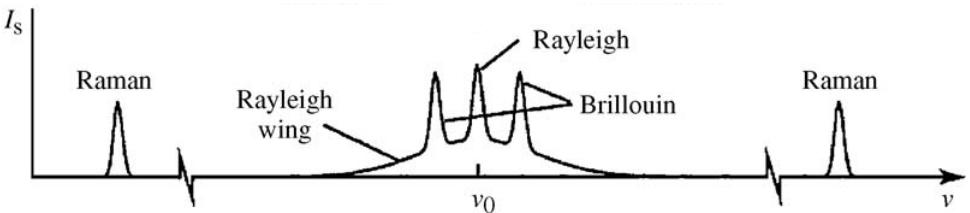
\includegraphics[width=0.75\linewidth]{figs/1-Intro/Boyd scattering frequency shift domains.png}
\caption{Relative domains of typical frequency shifts for Rayleigh, Rayleigh-wing, Brillouin, and Raman scattering.}
\label{fig:Introduction:scattering-domains}
\end{figure}

Returning to other optomechanical phenomena beyond scattering processes, the momentum of photons can exert forces on objects, leading to phenomena like radiation pressure, optical tweezing, and optical trapping. These effects are widely used in manipulating microscopic particles\cite{}, biological cells\cite{}, and atoms\cite{}, enabling studies of single molecules\cite{}, cold atoms\cite{}, and quantum computing elements\cite{}.

The final category of optomechanical interactions I will note here is that of nonlinear optical phenomena. Second harmonic generation, parametric oscillation, and four-wave mixing all feature the interaction between light and material nonlinearities that lead to the generation of new light frequencies.\cite{boyd2020nonlinear} The Kerr effect is the change in the refractive index of a material in response to an applied electric field, which can be induced optically with sufficient intensities of light. In general, nonlinear optical responses of materials are often only accessible with the use of high intensity laser light. This is emphasized by the fact that the field of nonlinear optics can be traced back to the discovery of second-harmonic generation in 1961\cite{franken1961generation}, just one year after the first demonstration of the laser by American physicist Theodor Maiman.\cite{maiman1960stimulated} These nonlinear effects provide the foundation for a range of technologies, including high-speed optical communication systems\cite{}, frequency converters\cite{}, and lasers for materials processing\cite{}.

Also included within nonlinear optical phenomena is electrostriction. Electrostriction is a reversible material deformation induced by an electric field, which can be generated by light in electro-optic materials. This effect is quadratic, scaling with the square of the applied electric field, and hence a nonlinear optical effect. At sufficiently high intensities, electrostrictive forces serve to enhance Brillouin scattering whereby the scattered light electrostrictively reinforces the acoustic wave that caused its scattering, leading to a nonlinear positive feedback loop known as \ac{SBS}. Photostriction is a related phenomenon that occurs when light absorption causes a change in the lattice structure of a material, leading to mechanical strain. It combines photovoltaic and piezoelectric effects and can be seen as an optically induced strain. These effects are utilized in designing optical modulators\cite{}, tunable photonic devices\cite{}, and smart materials that respond to light\cite{}.

In the remainder of this chapter I further describe the specific optomechanical phenomena that pertain to the research presented in this document: Brillouin scattering, electrostriction as it pertains to the \ac{SBS} process, and Raman scattering.


%%%%%%%%%%%%%%%%%%%%%%%%%%%%%%%%%%%
\section{Light Scattering}
\label{sec:Introduction:Light-Scattering}
Light scattering involves the redirection of light as a result of interactions with the constituent particles or molecules within a material medium. In every case, light scattering occurs because of variations in the material's optical properties. To understand why, envision a material with completely uniform particles---spatially and temporally consistent, or in other words, perfectly homogeneous. Figure \ref{fig:Introduction:homogeneous-material-no-scatter} shows an incident optical plane wave encountering a segment of such a material, denoted $\delta z$, containing a volume element $\delta V_{1}$. For any given incident wavelength $\lambda$ and any non-zero scattering angle $\theta$ at volume $\delta V_{1}$, there exists a corresponding volume element $\delta V_{2}$, located a distance $\frac{\lambda}{2\sin\theta}$ apart, which scatters light at the same angle $\theta$. The scattered waves from $\delta V_{1}$ and $\delta V_{2}$ would be out of phase by $\frac{\lambda}{2}$, leading to perfect destructive interference and no resultant scattered field. Thus, to achieve observable scattering, the material must possess inhomogeneities, allowing for variations in the optical properties between neighboring volumes. Fortunately, perfect homogeneity is not characteristic of real materials; all matter undergoes thermodynamic fluctuations at any temperature above absolute zero, and quantum fluctuations are inherent even at the ground state.

I now begin with a theoretical description of spontaneous light scattering as a result of thermodynamic fluctuations, presented in Boyd Nonlinear Optics.\cite{boyd2020nonlinear} This foundation will serve as a framework for understanding light scattering as specifically resulting from pressure variations (Brillouin scattering) as opposed to density variations (Rayleigh scattering). Later I will treat the case of higher-intensity \ac{SBS}. Ultimately I will build upon this theoretical basis to derive the coupled-wave equations of \ac{CABS}, a novel instrument which underpins many of my results. Let us build a theoretical description of light scattering considering thermodynamic fluctuations as the origin of the scattering process.

\begin{figure}[t] % here (h), at the top (t), at the bottom (b), or on a separate page for floats (p), in that preference order
\centering
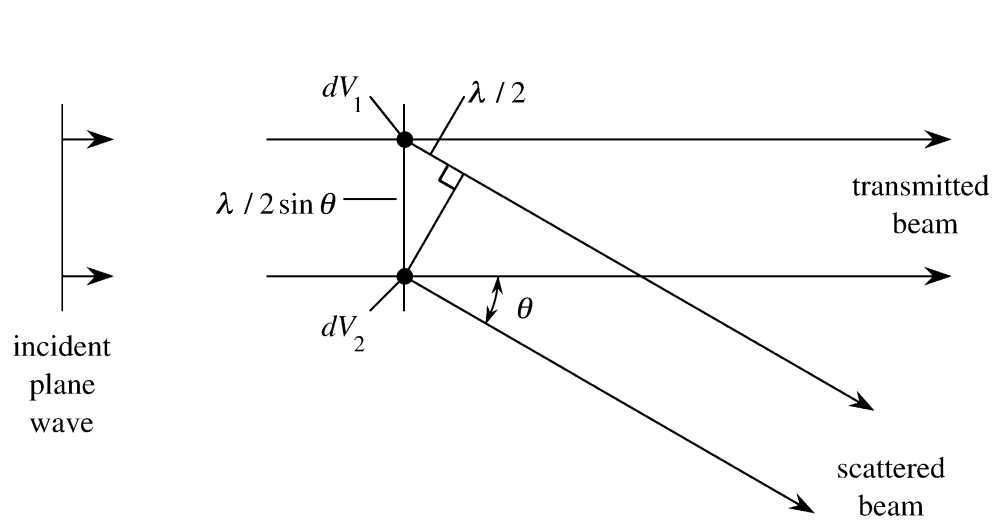
\includegraphics[width=0.75\linewidth]{figs/1-Intro/Boyd homogeneous material no scatter.png}
\caption{}
\label{fig:Introduction:homogeneous-material-no-scatter}
\end{figure}

\section{Spontaneous Brillouin Scattering}
\label{sec:Introduction:Spontaneous-Brillouin}
\lipsum[1]

\section{Stimulated Brillouin Scattering}
\label{sec:Introduction:Stimulated}
\lipsum[1]

\section{Phase-matching}
\label{sec:Introduction:Phase-matching}
\lipsum[1]

\section{Brillouin Gain of Materials}
\label{subsec:Introduction:Gain}
\lipsum[1]

\section{Raman Scattering}
\label{sec:Introduction:Raman}
\lipsum[1]

\section{Raman-like Brillouin Modes}
\label{sec:Introduction:Raman-like}
\lipsum[1]
